\documentclass[10pt, a4paper]{article}

\usepackage[paper=a4paper, left=1.5cm, right=1.5cm, bottom=1.5cm, top=1.5cm]{geometry}
\usepackage[utf8]{inputenc}
\usepackage[spanish]{babel}
\usepackage{graphicx}
\usepackage{multicol}
\usepackage[usenames,dvipsnames]{color}
\usepackage{amsmath}
\usepackage{verbatim}
\usepackage{footnote}
\usepackage{float}
\usepackage{amsfonts}
\usepackage{hyperref}
\usepackage{framed}
\usepackage{pdflscape}

\usepackage{pdfpages}

\usepackage{caratula}


\newcommand{\nota}[1]{
  $\bullet$ {\color{red}{#1}}
}


\materia{Ingeniería de Software II}

\titulo{TP 2 - Arquitectura}
\subtitulo{Grupo 9}

\integrante{Matías Nicolás Incem}{396/09}{matiasincem@gmail.com}

% Completen! - M.I.



\begin{document}

\maketitle
\tableofcontents
\newpage


\section{Introducción}

% Alguien va a tener que escribir algo acá. - M.I.

Este trabajo está centrado en una aplicación llamada \textit{Tweet-Rating}, que puede calcular el rating de distintos programas de televisión a partir de datos obtenidos de mensajes escritos en redes sociales, principalmente Twitter. Se presenta un diseño orientado a objetos del programa que realizaría esta tarea; por otro lado, se elaboró un prototipo del programa que puede verse en funcionamiento.

Para desarrollar el diseño y el código del programa el grupo se organizó a a partir de la metodología ágil conocida como \textit{SCRUM}, y se incluye en el trabajo la documentación de avances correspondiente a una iteración de trabajo.

%%%% ATRIBUTO DE CALIDAD %%%%

\newcommand{\QA}[8] {
\item
  Atributo de \textbf{#1}:\\\textit{``#2''}

  \begin{itemize}
  \item
    Fuente: #3
  \item
    Estímulo: #4
  \item
    Artefacto: #5
  \item
    Entorno: #6
  \item
    Respuesta: #7
  \item
    Medida: #8
  \end{itemize}

\vspace{10pt}
}

%%%%%%%%%%%%%%%%%%%%%%%%%%%%%

\section{Atributos de calidad}

% Descripción de atributos de calidad identificados, a través de escenarios, incluyendo prioridades relativas.

% %%%% PLANTILLA PARA ESCENARIO %%%%
% 
% \QA
%   {} % tipo de atributo
%   {} % texto del atributo
%   {} % fuente
%   {} % estímulo
%   {} % artefacto
%   {} % entorno
%   {} % respuesta
%   {} % medida de la respuesta
% 
% %%%%%%%%%%%%%%%%%%%%%%%%%%%%%%%%%%


  \begin{enumerate}

% 1- DISPONIBILIDAD

\QA
  {Disponibilidad} % tipo de atributo
  {Es fundamental garantizar que todos los nodos estarán siempre listos para procesar información a todo momento.} % texto del atributo
  {Interna del sistema} % fuente
  {Un nodo no responde a las consultas de los usuarios} % estímulo
  {Sistema} % artefacto
  {Operación normal} % entorno
  {Se reporta la falla y se solicita una reparación del nodo inhabilitado} % respuesta
  {El nodo vuelve a estar activo en el transcurso de una hora} % medida de la respuesta

\QA
  {Disponibilidad} % tipo de atributo
  {El sistema siempre debe estar disponible, aunque uno de los nodos no esté funcionando correctamente.} % texto del atributo
  {Externa} % fuente
  {No hay respuesta del nodo más cercano} % estímulo
  {Canal de comunicación} % artefacto
  {Normal} % entorno
  {Se pide información al nodo replicador} % respuesta
  {Se obtiene respuesta con demora menor que el doble del tiempo de respuesta normal} % medida de la respuesta

\QA
  {Disponibilidad} % tipo de atributo
  {La comunicación con el sistema de análisis de sentimiento SQPost suele fallar. Siempre que sea posible, se utilizará SQPost. En caso contrario, el sistema debe seguir respondiendo, y realizar el análisis con el sistema propio.} % texto del atributo
  {Interna del sistema} % fuente
  {Se recibe un timeout} % estímulo
  {Componente de SQPost} % artefacto
  {Normal} % entorno
  {Cambiar a modo de emergencia con análisis de sentimiento propio} % respuesta
  {El sistema no tarda más de 1 seg. en cambiar a modo de emergencia y continuar operando, desde que se descubrió la falla} % medida de la respuesta


% 2- PERFORMANCE

\QA
  {Performance} % tipo de atributo
  {Se espera que pueda procesarse una gran cantidad de imágenes obtenidas por la cámara del SmartTV.} % texto del atributo
  {Externa} % fuente
  {El SmartTV saca fotografías que serán tenidas en cuenta para mejorar el análisis del rating} % estímulo
  {Sistema de procesamiento de imágenes} % artefacto
  {Normal} % entorno
  {Se delega el procesamiento necesario al Hardware del SmartTV permitiendo una mayor descentralización y capacidad de cómputo} % respuesta
  {El sistema logra procesar para un determinado televidente una foto cada diez segundos} % medida de la respuesta

\QA
  {Performance} % tipo de atributo
  {El procesamiento de información deberá tardar menos de un segundo.} % texto del atributo
  {Externa} % fuente
  {El cliente hace un pedido de Rating o Popularidad} % estímulo
  {Sistema} % artefacto
  {Normal} % entorno
  {El sistema procesa el pedido y entrega una respuesta} % respuesta
  {El 90\% de las veces el pedido es respondido correctamente en menos de 1 segundo} % medida de la respuesta

\QA
  {Performance} % tipo de atributo
  {El sistema deberá responder efectivamente a 100 pedidos por segundo} % texto del atributo
  {Externa} % fuente
  {Varios clientes hacen pedidos en una ventana de 1 segundo} % estímulo
  {Sistema} % artefacto
  {Normal} % entorno
  {El sistema atiende los primeros pedidos de forma normal y pasa a modo sobrecargado, donde no responde ciertos pedidos hasta que se normalice la situación} % respuesta
  {El sistema responde 100 pedidos por segundo de forma normal} % medida de la respuesta

\QA
  {Performance} % tipo de atributo
  {El sistema responderá a un pedido de rating sin tener que acceder a redes sociales.} % texto del atributo
  {Externa} % fuente
  {Un cliente hace un pedido de rating para un programa} % estímulo
  {Sistema} % artefacto
  {Normal} % entorno
  {El sistema responde al pedido con información ya almacenada sin tener que hacer ningún pedido a redes sociales} % respuesta
  {El sistema responde al pedido al menos 10 veces más rápido que si debiera acceder a las redes sociales para responderlo} % medida de la respuesta


% 3- SEGURIDAD

\QA
  {Seguridad (Confidencialidad)} % tipo de atributo
  {La información que se transmite desde o hacia los nodos debe ser segura.} % texto del atributo
  {Atacante externo} % fuente
  {Captura un mensaje con información enviada desde o hacia un nodo, e intenta acceder a los datos confidenciales} % estímulo
  {Datos del sistema} % artefacto
  {Operación normal online} % entorno
  {El atacante no puede decodificar los datos} % respuesta
  {En el 99,9\% de los casos el atacante necesitaría más de 10 años para decodificar los datos} % medida de la respuesta

\QA
  {Seguridad (Integridad)} % tipo de atributo
  {La información que se transmite desde o hacia los nodos no debe poder alterarse desde afuera.} % texto del atributo
  {Atacante externo} % fuente
  {Captura un mensaje con información enviada entre nodos, lo altera y lo reenvía} % estímulo
  {Datos del sistema} % artefacto
  {Operación normal online} % entorno
  {El nodo descarta el mensaje adulterado y pide al emisor que se lo reenvíe} % respuesta
  {En el 98\% de los casos se puede identificar correctamente si un mensaje ha sido adulterado} % medida de la respuesta

\QA
  {Seguridad (Confidencialidad)} % tipo de atributo
  {La información almacenada dentro de los nodos debe ser segura.} % texto del atributo
  {Atacante externo} % fuente
  {Logra acceder a alguno de los repositorios de un nodo que contiene datos confidenciales} % estímulo
  {Uno de los respositorios de un nodo} % artefacto
  {Operación normal} % entorno
  {El atacante no puede decodificar los datos} % respuesta
  {En el 99,9\% de los casos el atacante necesitaría más de 10 años para decodificar los datos} % medida de la respuesta

\QA
  {Seguridad (Auditabilidad)} % tipo de atributo
  {Se desea almacenar los resultados de SQPost para poder mejorar el algoritmo propio de Sentiment Analysis.} % texto del atributo
  {Usuario común} % fuente
  {Pide el rating o la popularidad de un programa} % estímulo
  {Sistema} % artefacto
  {Operación normal online} % entorno
  {Se almacenan los resultados de aplicar el algoritmo SQPost y la consulta que generó cada uno} % respuesta
  {El 99,9\% de los resultados son almacenados} % medida de la respuesta


% 4- MODIFICABILIDAD

\QA
  {Modificabilidad} % tipo de atributo
  {El proyecto obtendrá datos de la actividad online de los usuarios, incluyendo varias redes sociales y comentarios en sitios de espectáculos. Se espera que periódicamente se agregue compatibilidad con nuevos sitios de Internet, sin perjudicar el uso de la aplicación.} % texto del atributo
  {Equipo de desarrollo} % fuente
  {Introduce un componente que obtiene datos de un determinado sitio de Internet y los procesa en el formato usado por el sistema} % estímulo
  {Sistema} % artefacto
  {Tiempo de ejecución} % entorno
  {El componente es agregado y empieza a funcionar, mientras el sistema continúa proveyendo los servicios normales} % respuesta
  {La incorporación del nuevo componente finaliza en menos de 20 horas de trabajo} % medida de la respuesta

\QA
  {Modificabilidad} % tipo de atributo
  {Es cada vez más importante el público multilingüe, por lo que debemos adaptarnos a la posibilidad de que mensajes en distintos idiomas se refieran a una misma emisión de un programa.} % texto del atributo
  {Administrador del sistema} % fuente
  {Quiere agregar soporte para un programa de TV en un nuevo idioma} % estímulo
  {Interfaz} % artefacto
  {En tiempo de ejecución} % entorno
  {Se realiza el cambio sin afectar el resto de la aplicación} % respuesta
  {Sólo se modifican los componentes correspondientes a los programas de TV} % medida de la respuesta

\QA
  {Modificabilidad} % tipo de atributo
  {Las personas que mejoraron nuestro algoritmo de sentiment analysis quieren aprender y mejorar la performance del mismo de manera continua.} % texto del atributo
  {Equipo de desarrollo de Sentiment Analysis} % fuente
  {Implementan un módulo nuevo o mejorado para realizar S.A. y lo incorporan al producto} % estímulo
  {Sistema} % artefacto
  {Tiempo de ejecución} % entorno
  {El software se intercambia de forma transparente al usuario y el producto sigue funcionando} % respuesta
  {El cambio se realiza en menos de 8 horas de trabajo y no se deben modificar otros elementos del sistema} % medida de la respuesta


% 5 - USABILIDAD

\QA
  {Usabilidad} % tipo de atributo
  {Se quiere tener una interfaz bonita y fácil de usar, para tener mayor aceptación entre el público.} % texto del atributo
  {Usuario de la aplicación} % fuente
  {Desea ver el rating actual de un programa de TV} % estímulo
  {Sistema} % artefacto
  {En tiempo de ejecución} % entorno
  {Se provee una interfaz de usuario fácil de entender y usar} % respuesta
  {El 90\% de los usuarios puede realizar la operación al usar por primera vez la aplicación, y demoran menos de 30 segundos} % medida de la respuesta
  

\end{enumerate}




\section{Arquitectura}

% Documento que describa las principales decisiones de arquitectura que fueron evaluadas y la decisión que se tomó en cada caso. Se deberá incluir una o más vistas que describan la visión general de cómo será el producto en el nivel de la arquitectura.

\subsection{Vista principal de componentes y conectores}

\begin{figure}[H]
\centering
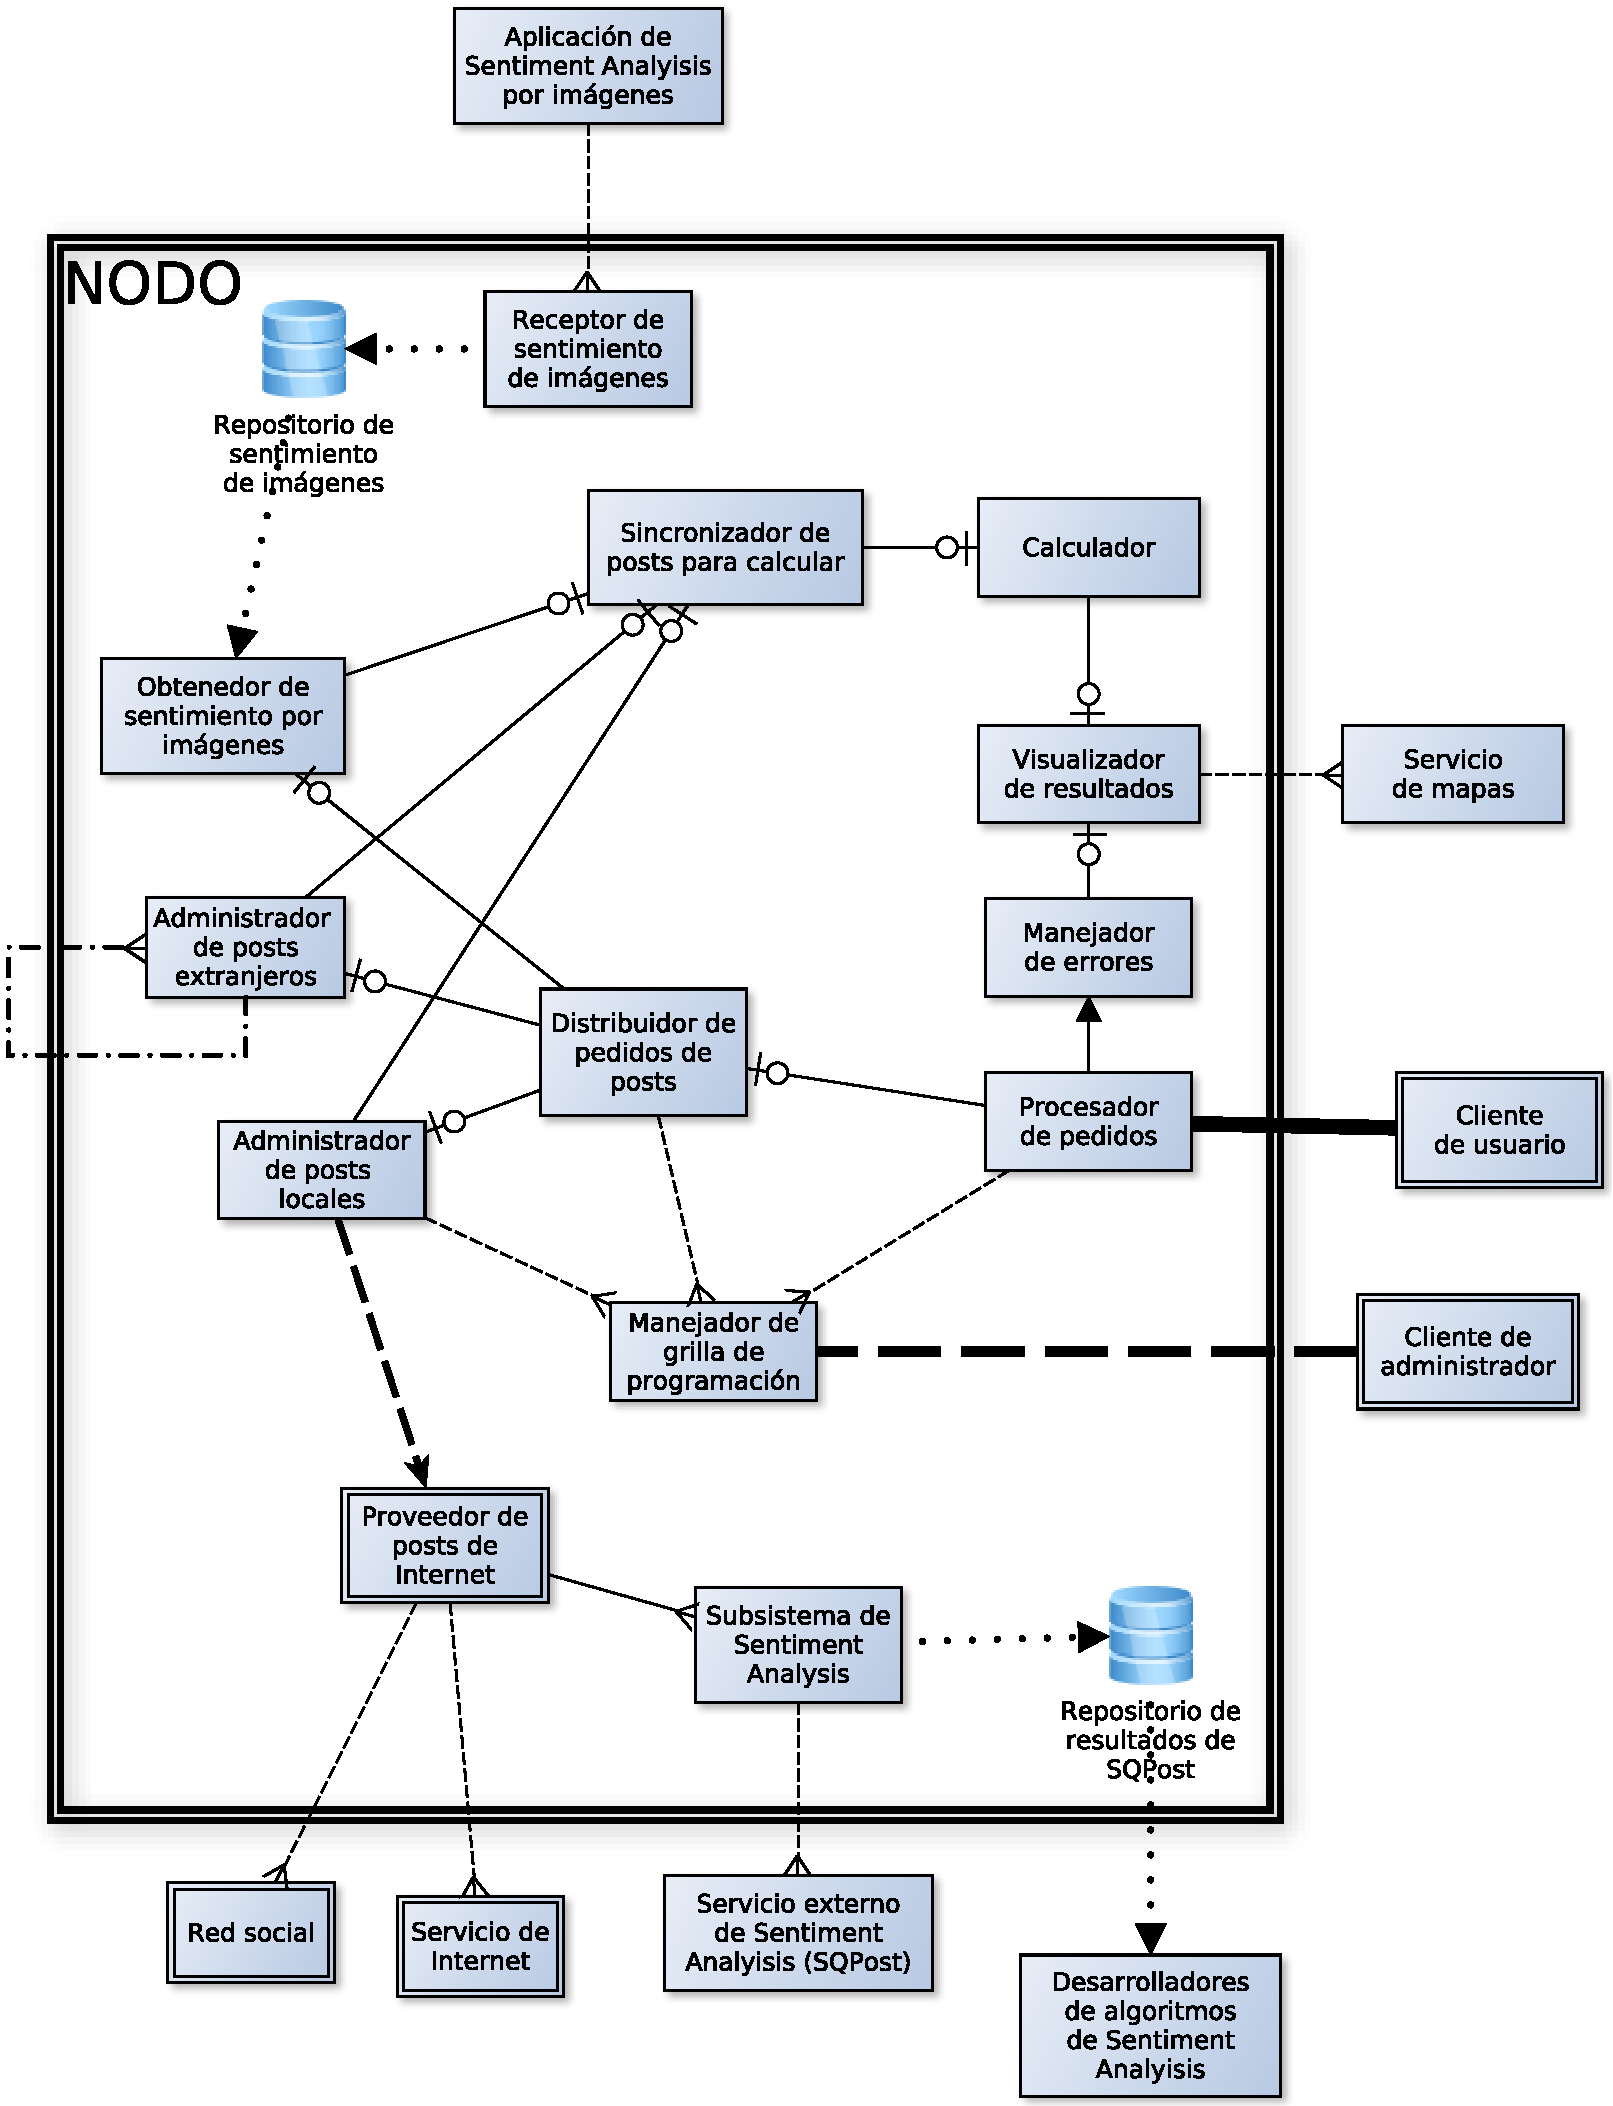
\includegraphics[width=\textwidth]{graph/main.pdf}
%\caption{Post Filterer}
\end{figure}

\begin{figure}[H]
\centering
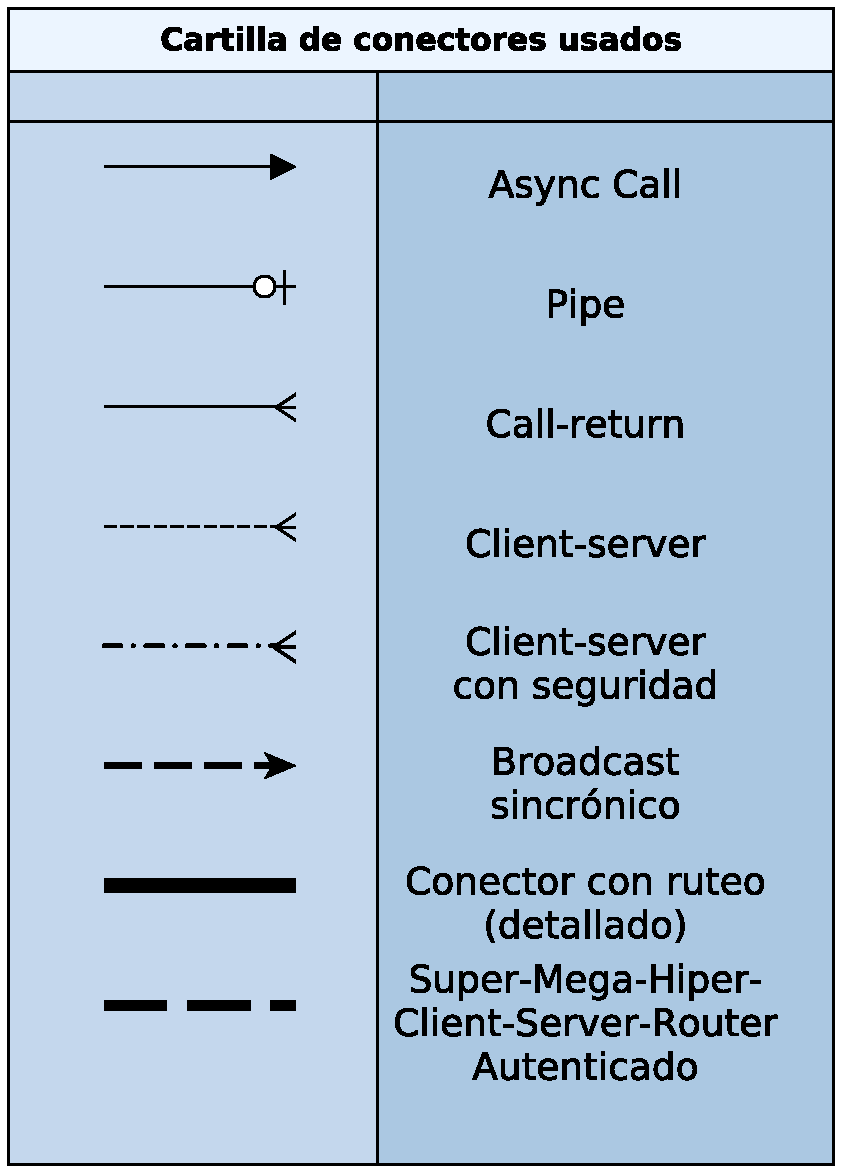
\includegraphics[width=0.5\textwidth]{graph/cartilla.pdf}
%\caption{Post Filterer}
\end{figure}


\subsection{Conector que rutea pedidos}

\begin{figure}[H]
\centering
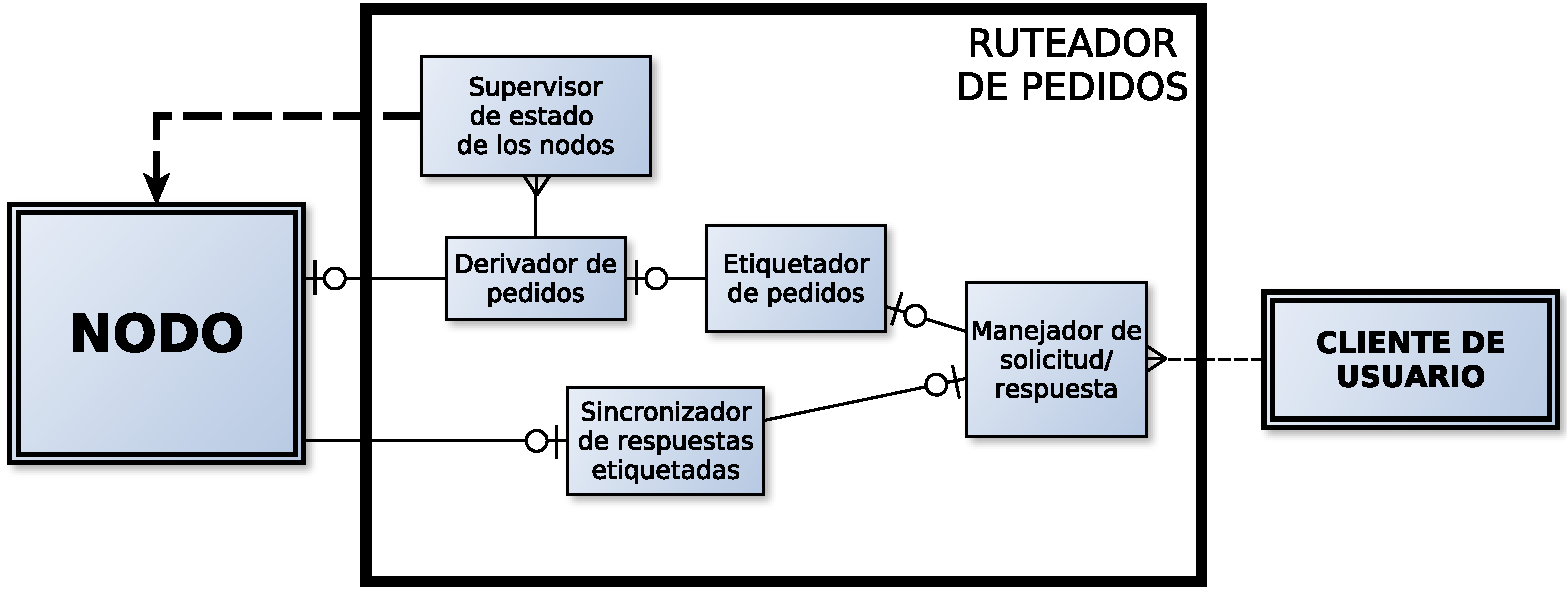
\includegraphics[width=\textwidth]{graph/conector.pdf}
%\caption{Post Filterer}
\end{figure}

El cliente se conecta a un servidor web a través de la página de internet del sistema y realiza un pedido. Este pedido debe viajar al nodo más cercano geográficamente a su ubicación. Para esto primero debe pasar por un ruteador de pedidos para que lo diriga.
El pedido llega al manejador, quien mantiene abierta la comunicación con el cliente hasta que llegue la respuesta. El pedido, luego, es etiquetado tal que el resto de los componentes puedan identificarlo a lo largo del flujo de datos. El derivador de pedidos indentifica la IP correspondiente al mismo y la vincula con el nodo al que debería ir. Luego, verifica el estado de dicho nodo y envía el pedido. Si no está activo, entonces, lo envía al siguiente nodo más cercano.

El supervisor de estado es un componente que controla períodicamente si los nodos están activos. Si detecta que algún nodo no responde avisa a los responsables a mediante el envío de un email, para que sea reparado.

Cuando llega la respuesta el sincronizador se encarga de asociarla con el cliente correspondiente utilizando su etiqueta. De esta forma el manejador puede devolver la respuesta al cliente y cerrar la conexión.

Es importante destacar que el ruteador de pedidos está replicado, de manera que siempre que deje de responder puede ser reemplazado inmediatamente y seguir operando. Es vital mantener este componente en funcionamiento ya que sin él no puede realizarse la comunicación con los servidores.


\subsection{Conexión de administrador}

Los administradores del sistema son usuarios especiales que tienen acceso a la grilla de programación, para agregar, eliminar o modificar los programas de TV que el sistema conoce, así como sus características y propiedades. El administrador se conecta directamente a uno de los nodos y edita los programas de TV del área correspondiente a dicho nodo. La conexión se realiza de forma segura, y el administrador debe estar autenticado para poder operar.


\subsection{Procesador de pedidos}

\begin{figure}[H]
\centering
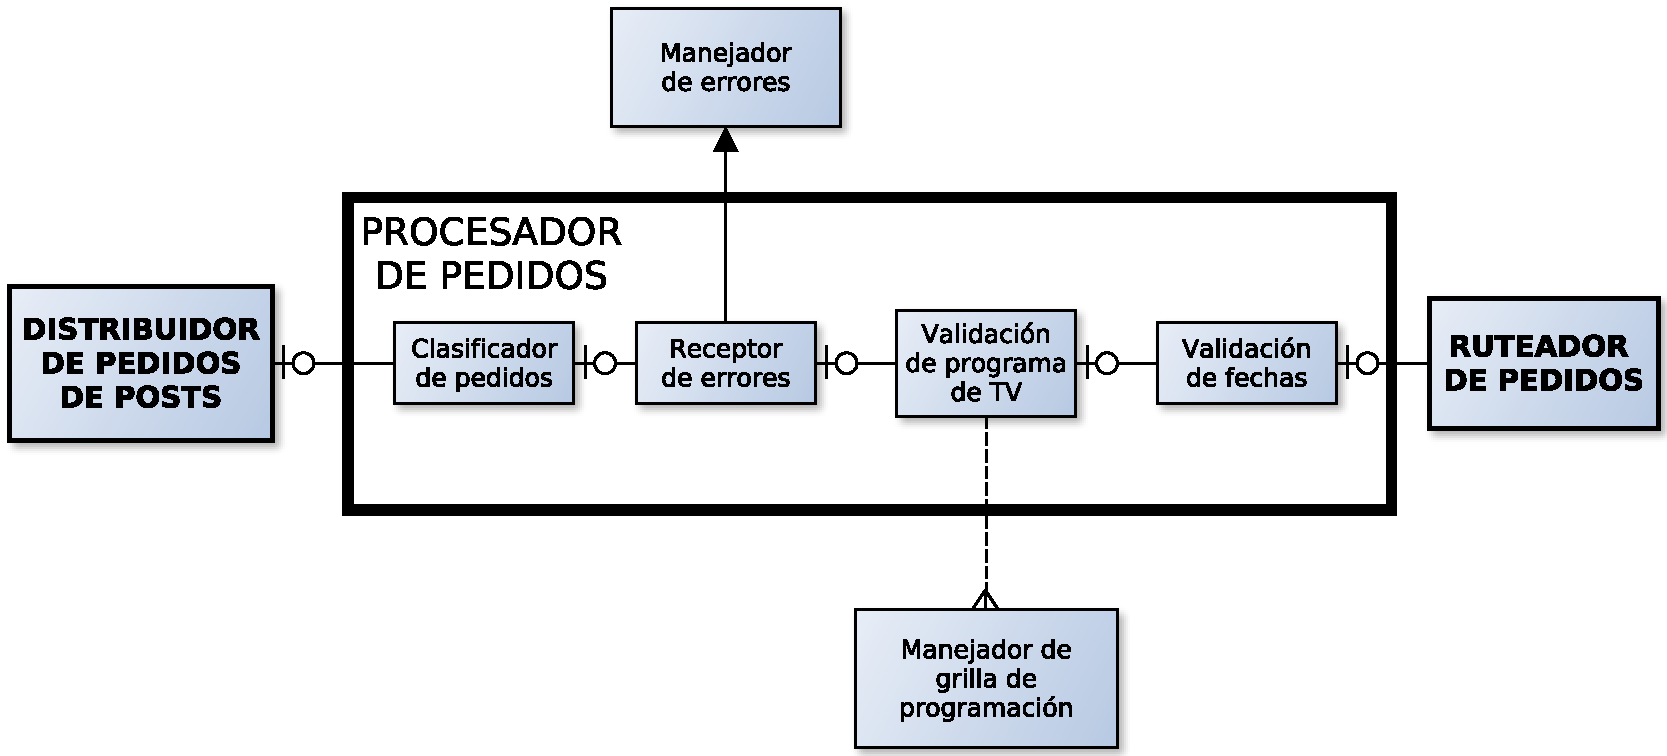
\includegraphics[width=\textwidth]{graph/procpedidos.pdf}
%\caption{Post Filterer}
\end{figure}

Cuando llega un pedido de un usuario de la aplicación al nodo, este componente lo recibe y verifica que las fechas ingresadas tengan un formato válido y que 
además correspondan a un tiempo válido que se pueda consultar. En el caso de que se haya ingresado un intervalo de tiempo, se verifica que este bien constituido (que el inicio sea anterior al final). Luego se verifica que el programa de televisión pedido sea parte de la grilla del sistema, para lo cual se consulta al manejador de la grilla de programación. Si el pedido falla alguno de estos test se envía un mensaje de error que se propaga hasta el receptor de errores quien envía dicho mensaje al manejador de errores para que lo muestre por pantalla. Si el pedido no es filtrado en esta instancia, entonces, pasarña por el clasificador de pedidos que lo etiqueta como pedido de Rating o Popularidad. Una vez hecho esto, se encola el pedido en el distribuidor de pedidos de posts.

\subsection{Distribuidor de pedidos de posts}

\begin{figure}[H]
\centering
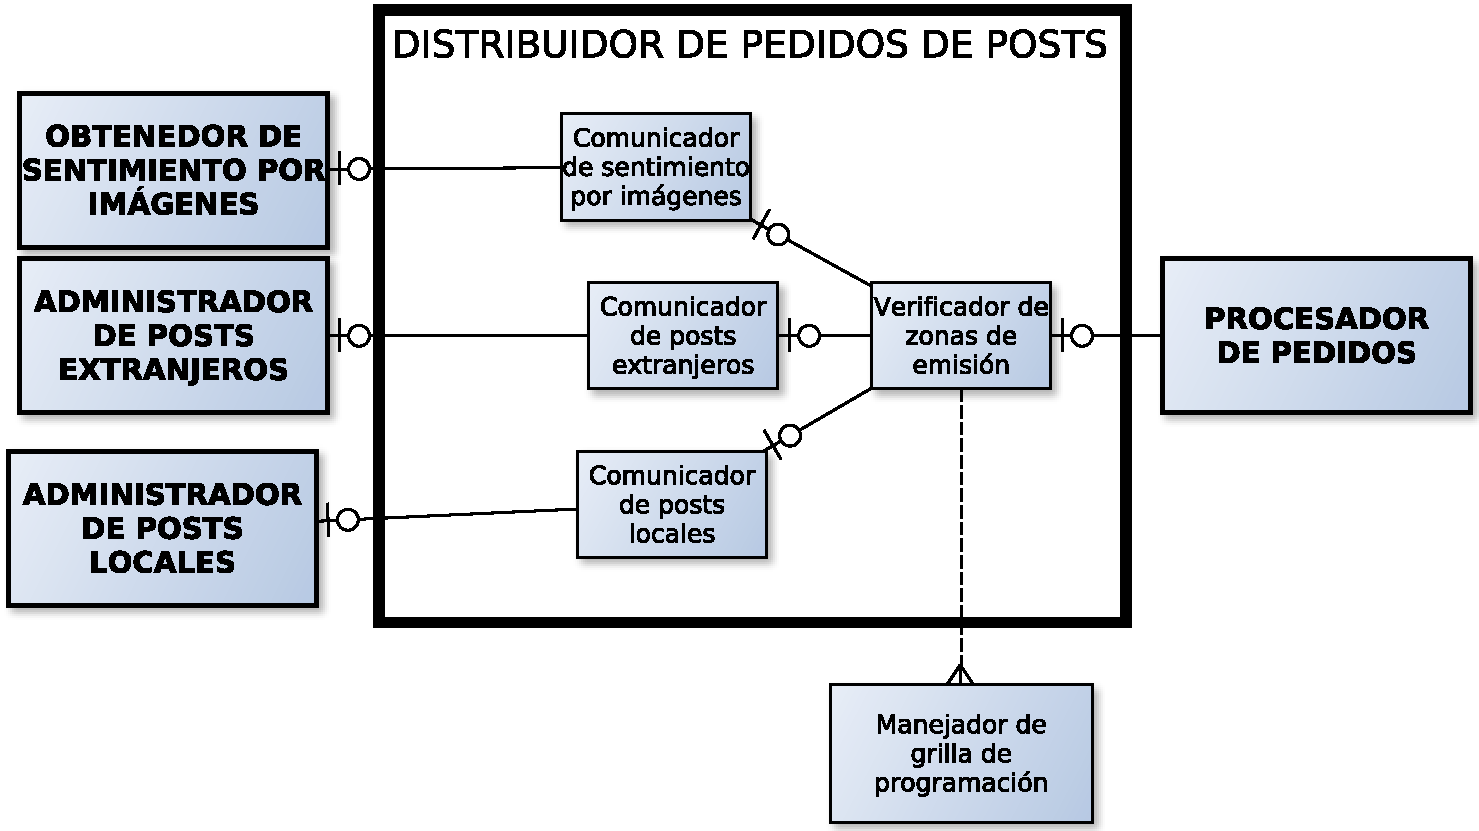
\includegraphics[width=\textwidth]{graph/distribuidor.pdf}
%\caption{Post Filterer}
\end{figure}

Este componente tiene la responsabilidad de pedir los posts necesarios para resolver el pedido del usuario. En primer lugar, se etiqueta el pedido según su precedencia: del mismo nodo o de otro nodo. Esto servirá para enviar los resultados a quien los necesite. Luego, se verifica la zona de emisión del programa que fue solicitado para saber si necesita conseguir posts de otras regiones (manejadas por otros nodos) y si necesita posts locales. Se conecta con los comuinicadores para hacer los pedidos correspondientes.

\subsection{Administrador de posts locales}

\begin{figure}[H]
\centering
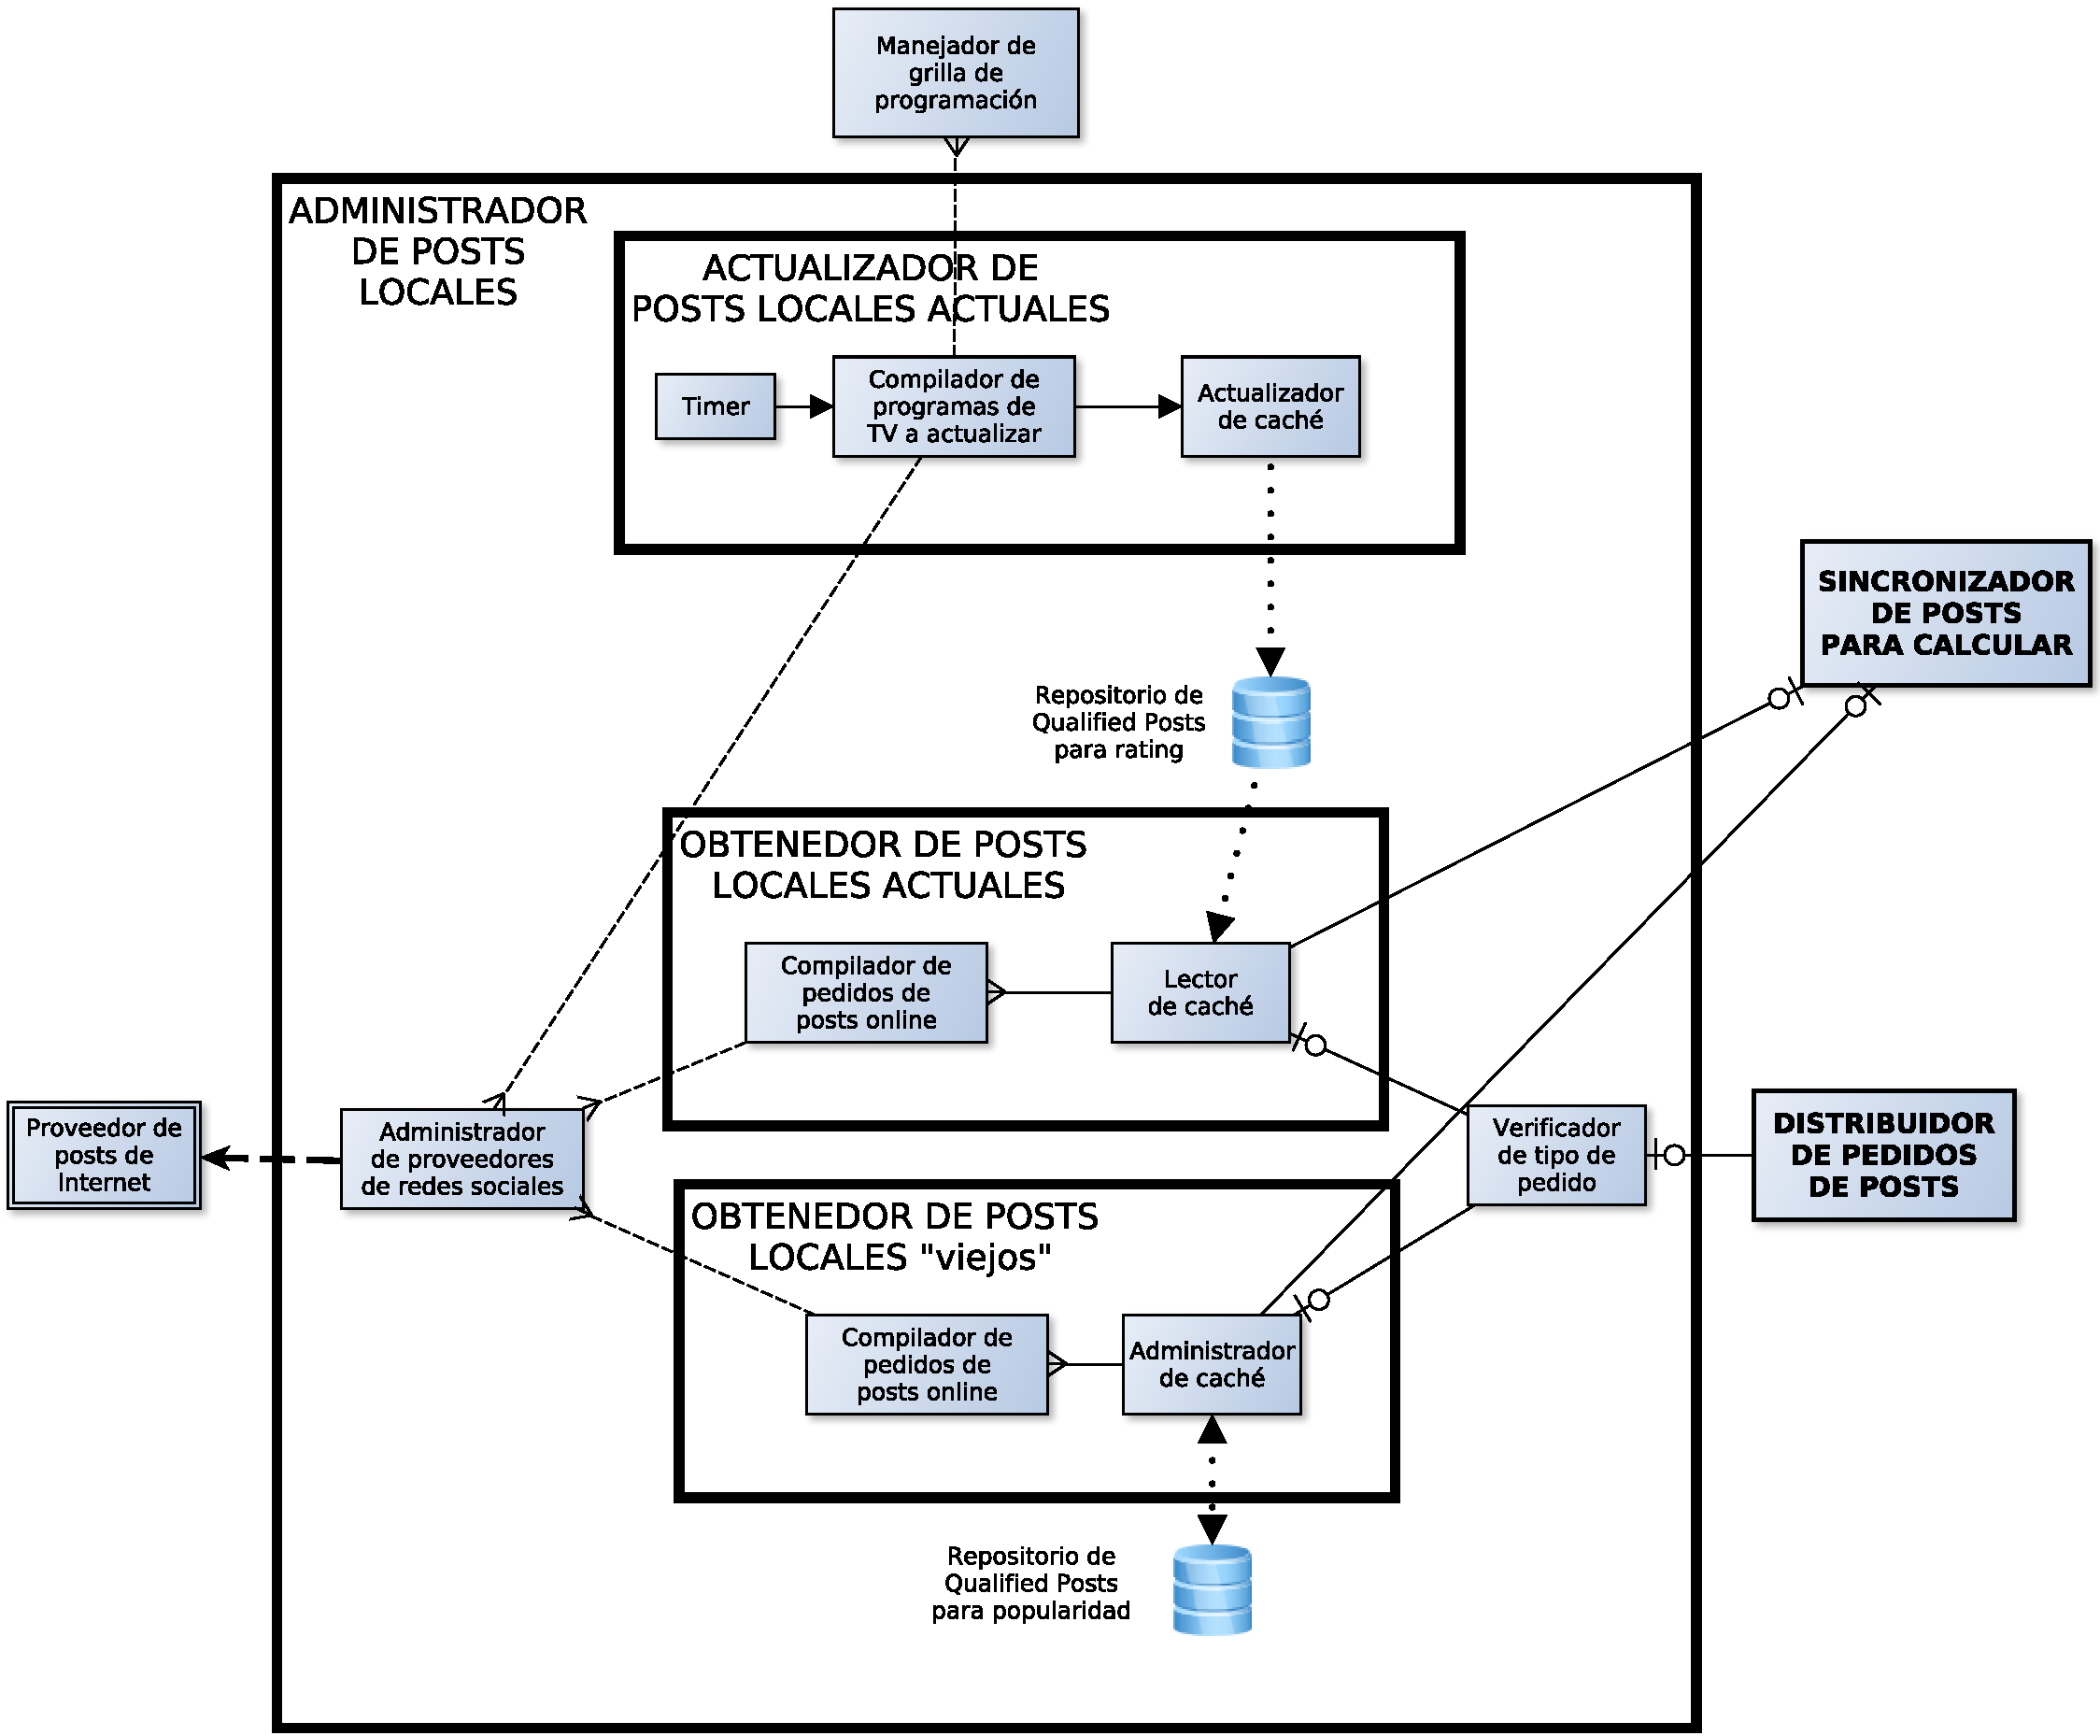
\includegraphics[width=\textwidth]{graph/adminlocal.pdf}
%\caption{Post Filterer}
\end{figure}

Cuando llega un pedido de post a este componente lo primero que se hace es verificar si es un pedido de rating o popularidad. 
Si es un pedido de rating, el obtenedor de post locales actuales revisa la caché correspondiente al ratingpara obtener los posts que necesita, si no los encuentra hace un llamada al compilador de pedidos de posts online. Este organiza el pedido que debe hacerse a las redes sociales y servicios de internet y le envía dicho pedido al administrador de proveedores. Este administrador conoce a cada uno de los proveedores y cada uno de ellos puede conectarse a un determinado sitio de internet. El administrador le pasa el pedido a todos los proveedores. Cada uno de ellos busca en su sitio de internet y responde con qualified posts. Luego, el administrador reúne todos los resultados y los devuelve al compilador de pedidos de posts online, que a su vez los devuelve al lector de caché. En este momento el lector caché tiene los resultados del rating correspondientes al nodo local, y se distribuirán a quien los haya pedido. Si fue una consulta local, los datos pasarán a ser sincronizados con los otros resultados. Si fue 
una consulta proveniente de otro nodo, se enviarán a dicho nodo.

Si es un pedido de popularidad, se envía al obtenedor de posts locales de popularidad, que posee un funcionamiento similar, con una diferencia: si recibe datos provenientes de Internet, los guarda en la caché de popularidad.

Con respecto a la caché del rating, esta se actualizará constantemente según los programas que estén al aire. La actualización de la caché no depende de los pedidos de rating que se realicen. Es esperable que los pedidos de rating siempre puedan encontrarse en la caché, siempre que esta esté disponible.
La caché de popularidad, en cambio, se actualizará a medida que se realicen pedidos con algún método que priorice las búsquedas más frecuentes. No podemos pretender que los resultados de las búsquedas estén siempre en caché debido a que hay un gran número de consultas posibles, por lo tanto será habitual que para este tipo de pedidos se acceda a las redes sociales. 

\subsection{Administrador de posts extranjeros}

\begin{figure}[H]
\centering
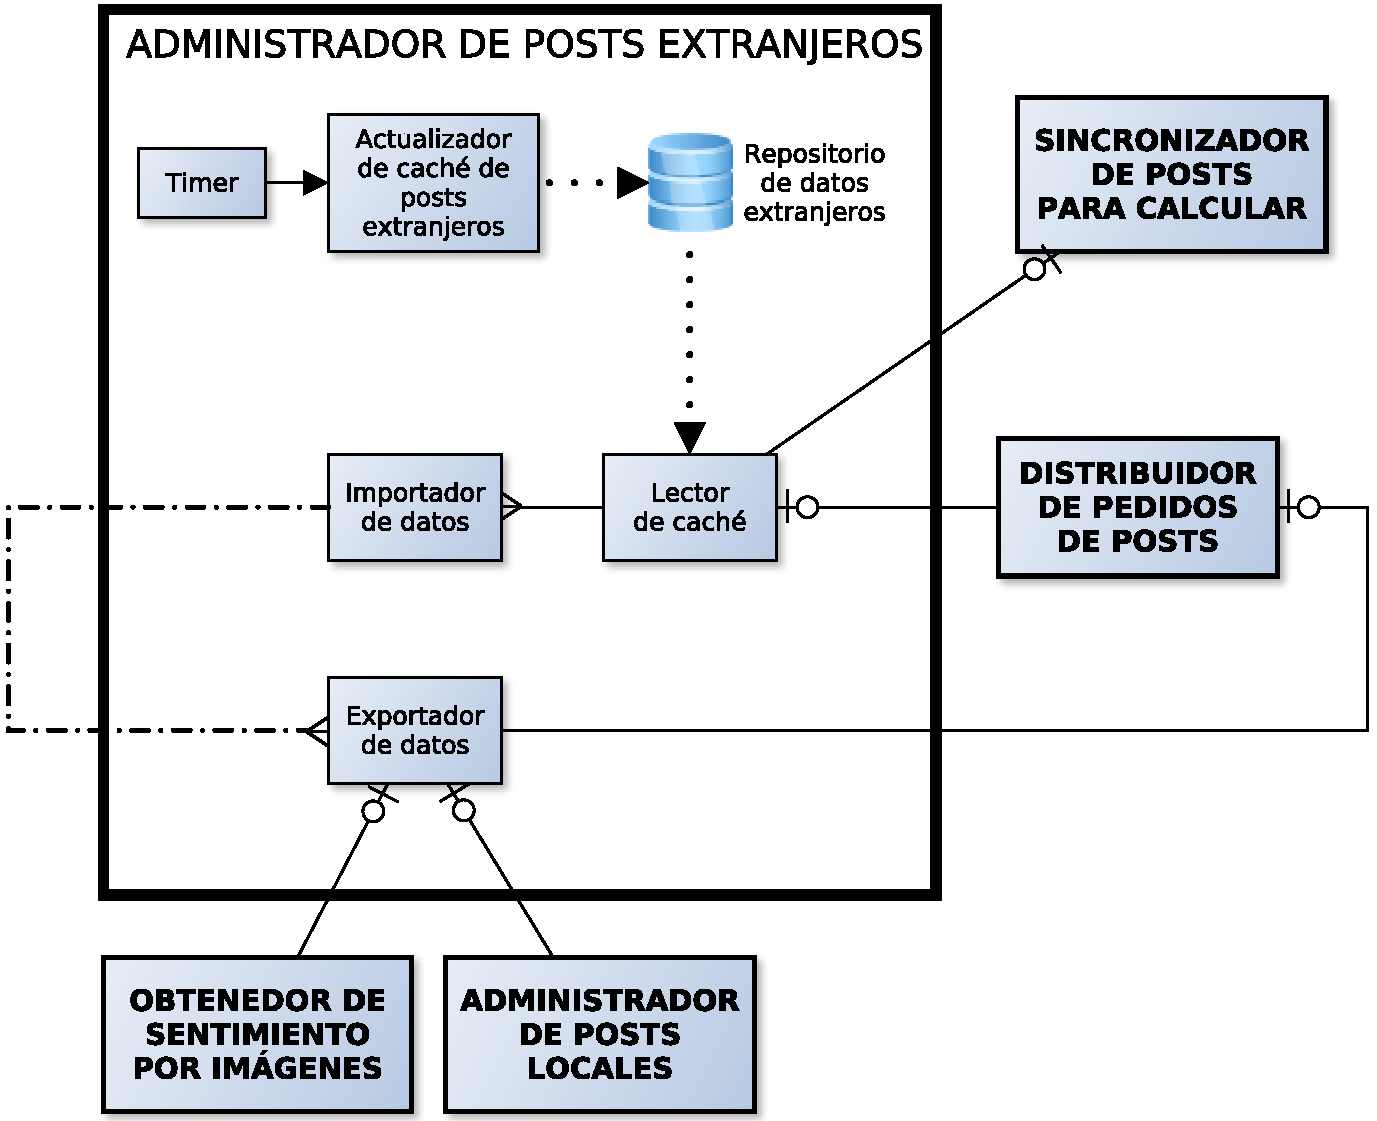
\includegraphics[width=0.8\textwidth]{graph/administradorPostsExtranjeros.pdf}
%\caption{Post Filterer}
\end{figure}

Una vez que el distribuidor encuentra un pedido que requiera la comunicación con otros nodos, el administrador de posts extranjeros será el encargado de obtener la respuesta. Antes de explicar este componente es necesario aclarar que el cada nodo tiene replicado a otro nodo en su totalidad, por lo que cuando se pidan posts que se corresponden a otros nodos, primero se realiza un búsqueda en este repositorio réplica en el nodo local. Si la búsqueda es exitosa, entonces se comunica la respuesta al sincronizador de posts para calcular. En otro caso, el pedido se realiza al importador de datos. Este es el componente que se comunica efectivamente con el nodo necesario, mediante una comunicación cliente-servidor de forma segura. El pedido es recibido por el Exportador de datos, quien lo encola en el distribuidor de pedidos, pero ahora referido al nodo extranjero. Luego se etiqueta como un pedido proveniente de un nodo extranjero y se envía a los componentes correspondientes para completar la respuesta. Esta vuelve 
al exportador de datos desde el obtenedor de sentimientos por imágenes y el administrador de posts locales, para finalmente regresar al primer nodo, al importador de datos, al lector de caché y luego al sincronizador.


El repositorio de datos extranjeros, como habíamos dicho, replica los datos de uno de los nodos, para asegurarnos de que al momento que se caiga cualquiera de los mencionados, entonces el sistema siga funcionando. Por ello, cuando esto pase se pasará a una condición degradada del sistema y la cantidad de pedidos resuletos por minuto se verá disminuída. Para mantener este repositorio sincronizado períodicamente el actualizador de post extranjeros hará los pedidos necesarios.

\subsection{Subsistema de Sentiment Analyisis}

\begin{figure}[H]
\centering
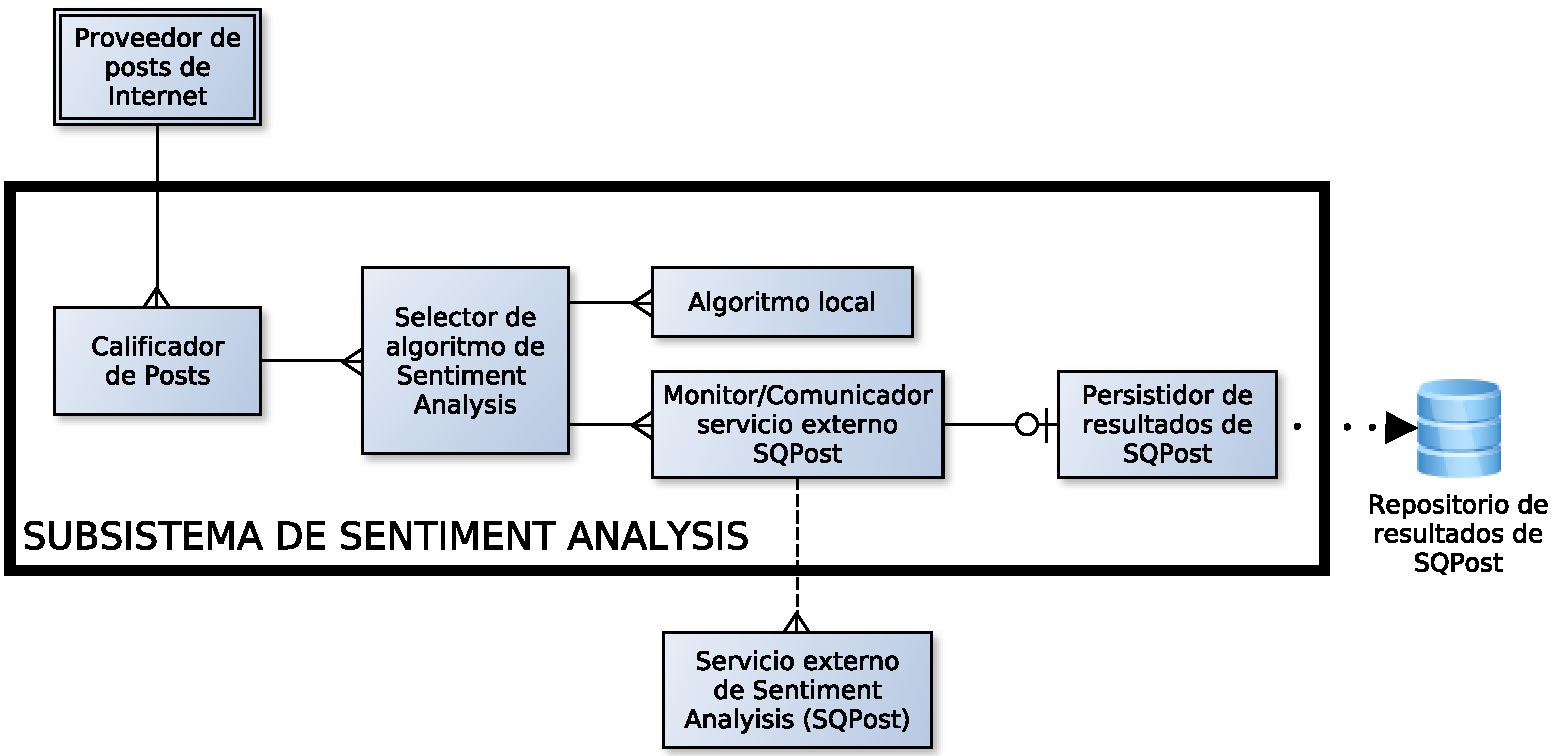
\includegraphics[width=0.8\textwidth]{graph/subsistemaSentimentAnalysis.pdf}
%\caption{Post Filterer}
\end{figure}

El componente de Sentiment Analysis se utiliza para asignarle un sentimiento a cada post que se almacena en el sistema. Cuando un proveedor de posts, vinculado a una determinada red social, obtiene mensajes de dicho sitio y los ingresa al sistema en el formato de post, hace una llamada al Sentiment Analyisis para que los califique. El calificador recibe y organiza los posts, y se conecta con el selector de algoritmo para realizar la calificación propiamente dicha. El selector intenta comunicarse con el servicio externo, que se considera como el más confiable en cuanto a precisión de resultados pero no en disponibilidad. Si recibe una respuesta del servicio, devuelve los sentimientos obtenidos, mientras el persistidor se encarga de almacenarlos en el repositorio para futuros análisis. Si no la recibe, intenta con el algoritmo interno del sistema.

Cuando tiene una respuesta proveniente de alguno de los algoritmos, el calificador convierte los posts obtenidos en posts calificados, y los devuelve para que el proveedor de posts pueda responder la consulta que le habían realizado.


\subsection{Aplicación de Sentiment Analyisis por imágenes}

\begin{figure}[H]
\centering
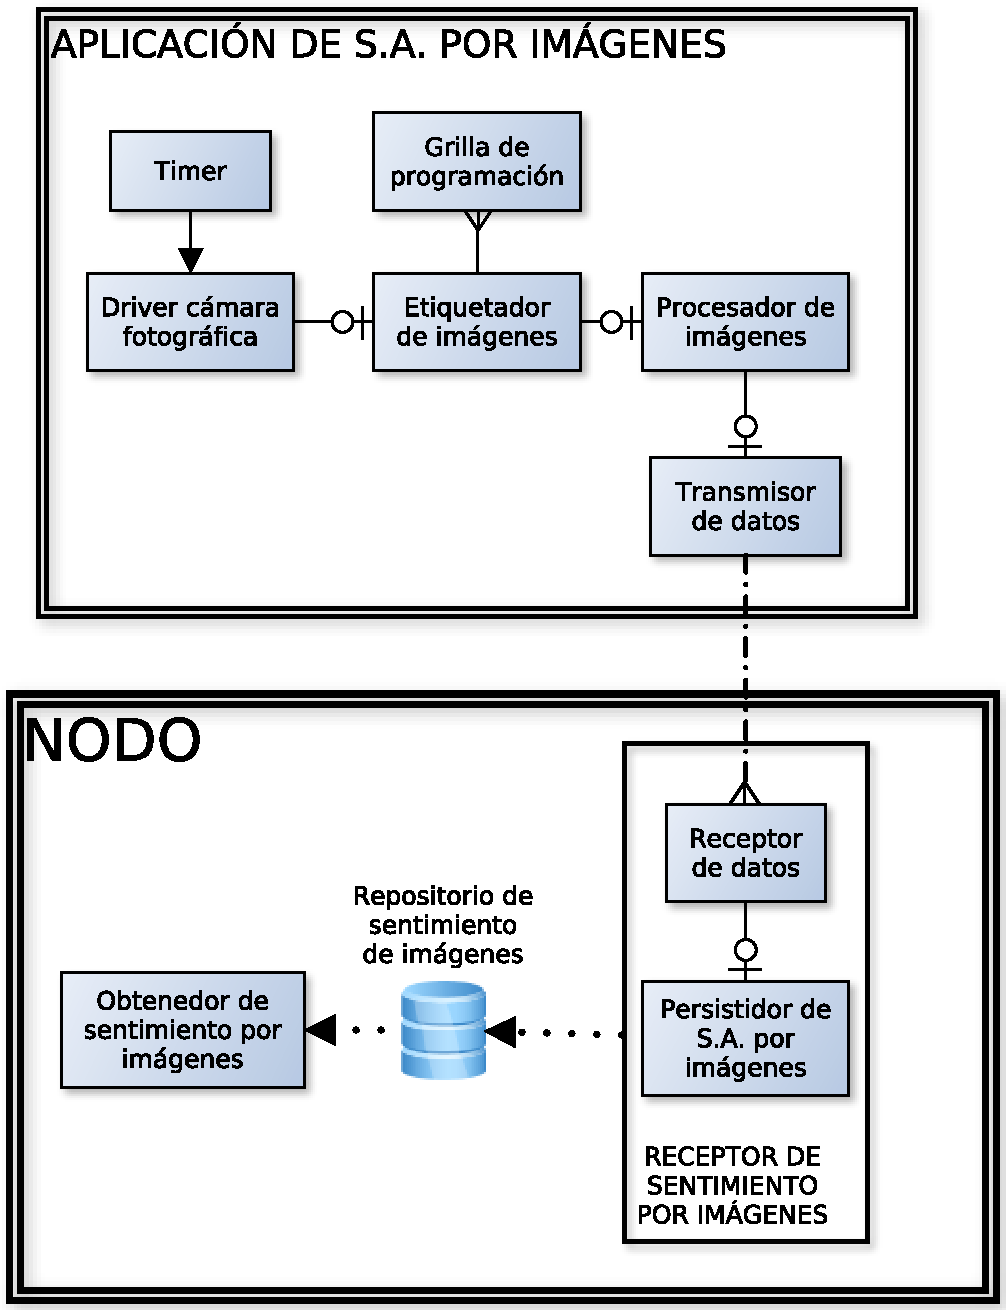
\includegraphics[width=0.7\textwidth]{graph/smarttv.pdf}
%\caption{Post Filterer}
\end{figure}

El sentiment analyisis por imágenes es una funcionalidad del sistema que se agrega a la obtención de datos a través de posts, y ofrece mayor cantidad de datos para operar. La aplicación funcionará en su mayor parte fuera de los nodos, distribuida entre los sistemas de los clientes que ofrecen datos. (Es decir, se ejecutará dentro de los Smart TVs de los usuarios que activen el producto.) El sistema es activado por un timer, que periódicamente indica al driver de la cámara fotográfica del dispositivo que tome una foto y la ponga en cola para procesarla. El procesamiento comienza con el etiquetado de la información, en el cual se le agrega un timestamp y el programa de TV que se está mirando (que un televisor digital puede obtener a partir de la grilla). Luego se procesa la foto en sí, y se obtiene la información de número de personas mirando y datos de cada una, así como su sentimiento respecto del programa de TV.

Los datos anónimos obtenidos de las imágenes se transmiten al nodo a través de una comunicación segura, con encriptación, y se retorna un ACK. La aplicación que está incluida en los televisores de una región está programada para comunicarse directamente con el nodo correspondiente a dicha región; si el nodo en algún momento está inactivo, se dejará temporalmente de recibir datos de imágenes para esa zona. Dentro del nodo, el persistidor de datos se encarga de guardar los datos recibidos para ser usados en futuras consultas.

\subsection{Obtenedor de Sentiment Analyisis por imágenes}

\begin{figure}[H]
\centering
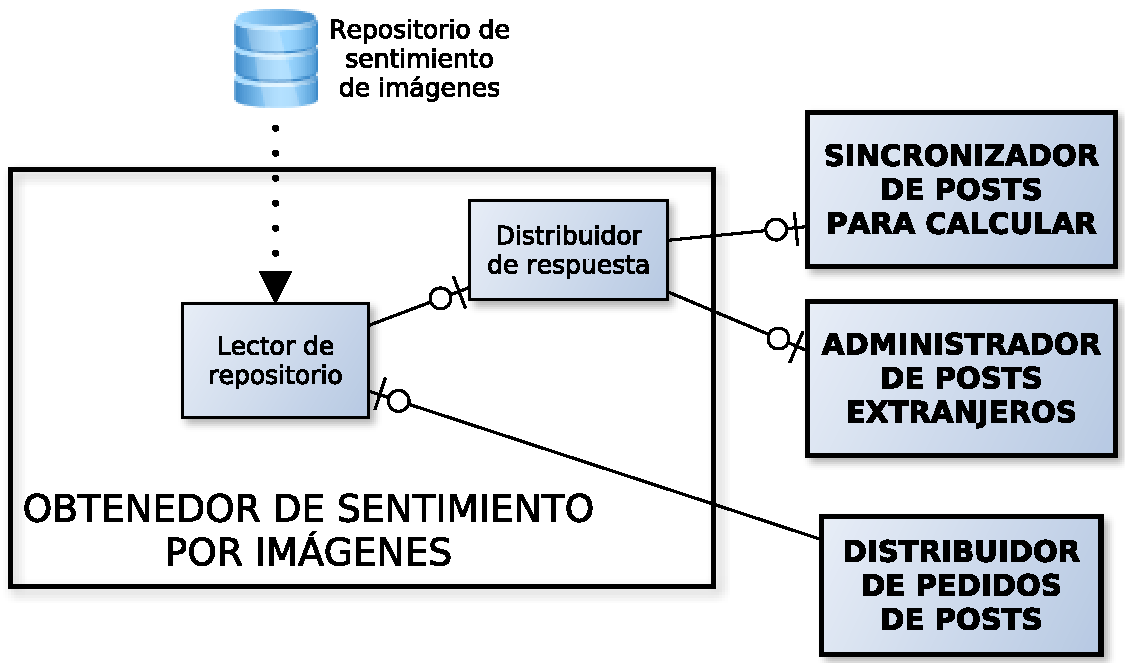
\includegraphics[width=0.7\textwidth]{graph/obtenedorimg.pdf}
%\caption{Post Filterer}
\end{figure}

El Obtenedor de sentimiento por imágenes es uno de los recursos para obtener datos para un pedido. El distribuidor de pedidos de posts le informa cuando llega un pedido, que puede provenir desde el mismo nodo o de otro. El lector de repositorio encuentra los datos que necesita para cumplir el pedido, y el distribuidor de respuesta los envía a quien los necesita, según la etiqueta que tenía el pedido.

\subsection{Sincronizador}

\begin{figure}[H]
\centering
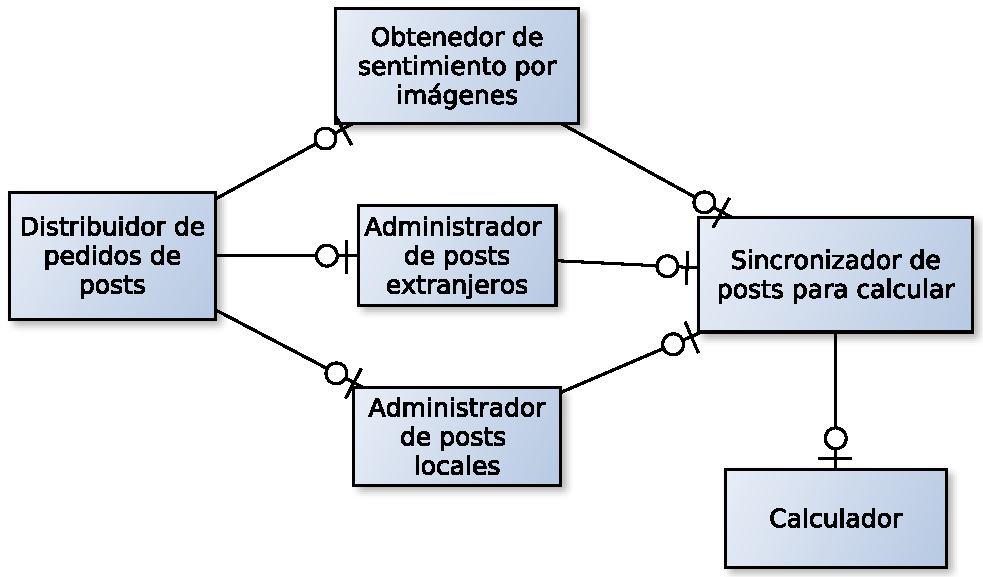
\includegraphics[width=0.7\textwidth]{graph/sincro.pdf}
%\caption{Post Filterer}
\end{figure}

El sincronizador recibe datos de tres fuentes distintas: posts locales, es decir, del área correspondiente al nodo que está ejecutando el pedido; posts extranjeros, que fueron procesados y calificados en los nodos de otras áreas, y sentimiento por imágenes, que proviene del sistema externo y trae sentimientos, pero no mensajes. Todos esos datos deben reunirse para cada pedido. Es posible sincronizar todos los datos del mismo pedido gracias a las etiquetas que se aplican al principio del flujo del sistema, las cuales identificana quién pertenece cada dato. Cuando las tres fuentes comunican que ya enviaron todos los datos posibles para un pedido determinado, el sincronizador los envía al calculador para que los procese.

\subsection{Visualizador de resultados}

\begin{figure}[H]
\centering
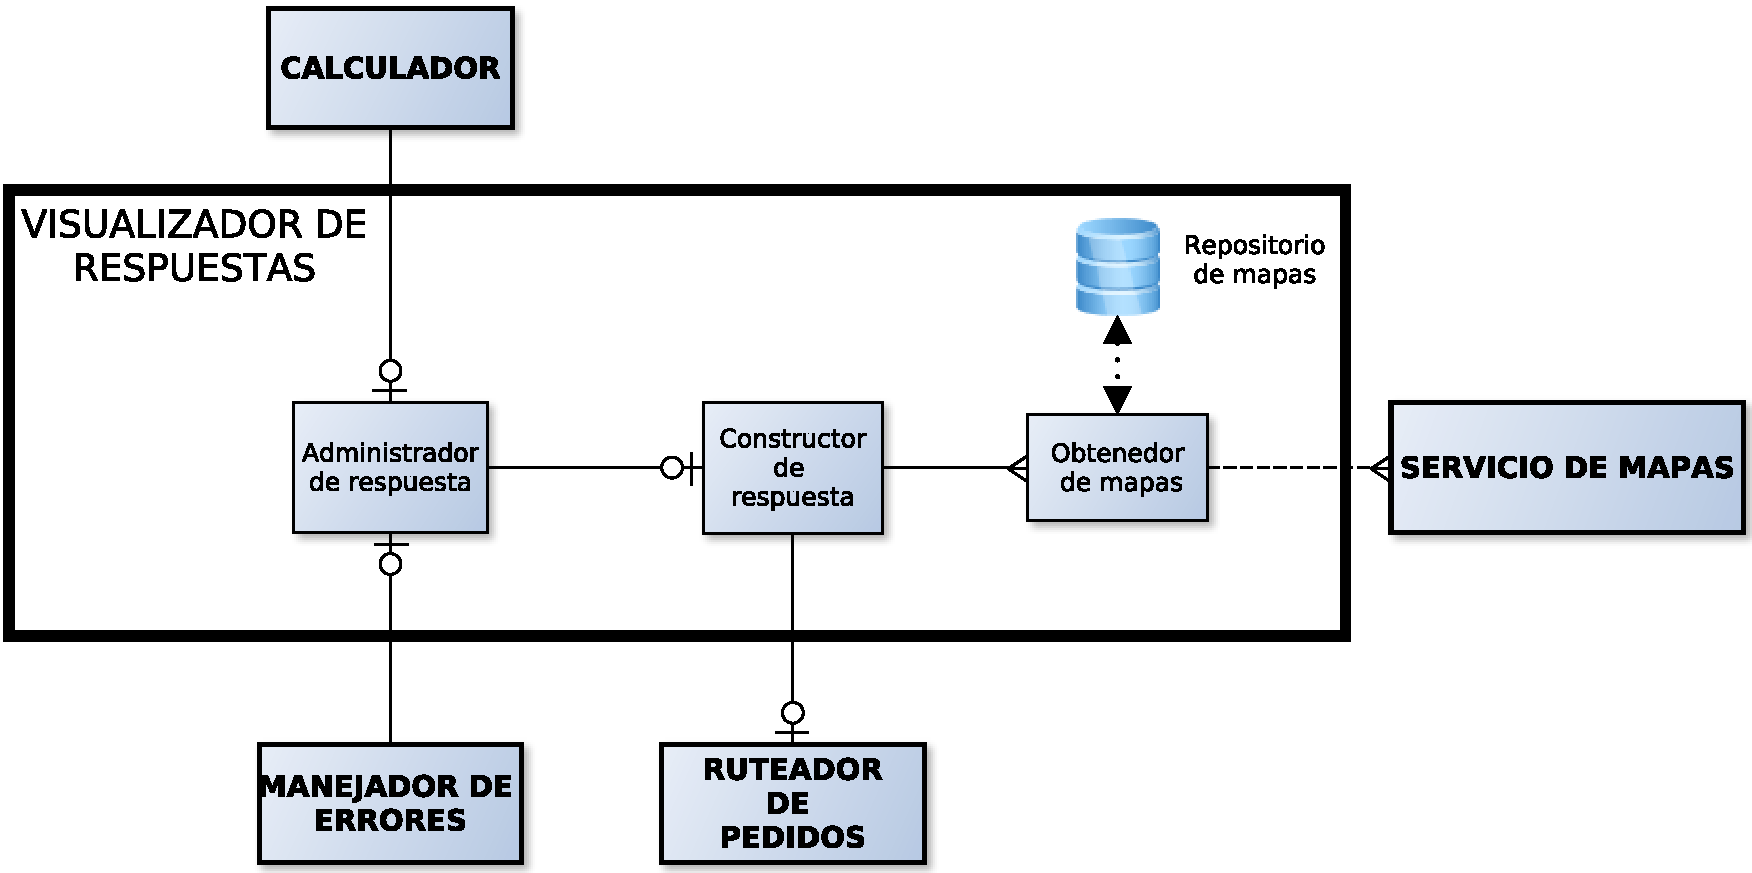
\includegraphics[width=\textwidth]{graph/visualizador.pdf}
%\caption{Post Filterer}
\end{figure}

El visualizador de resultados se encarga de darle formato a la respuesta que recibirá el cliente, ya sea un resultado de rating o popularidad, un mensaje de error, debido a que la consulta del cliente fue invalidada en algún momento por el procesador de pedidos, o un mapa donde se visualizan los resultados. Para ello, el visualizador cuenta con un administrador cola de resultados. A medida que se van desencolando dichos mensajes, estos son comunicados al constructor de respuesta, que se encarga de darles el formato correspondiente según la UI que se esté utilizando o, por ejemplo, un correcto mensaje de error. También se puede comunicar con el obtenedor de mapas, quien provee de un mapa, ya sea buscándolo en repositorio local o en algún servicio de internet como Google Maps. Tal vez este repositorio no sea de tanta utilidad debido al cambio constante del rating, pero tal afirmación habría que hacerla luego de un análisis estadístico de los pedidos de los usuarios. Por último, se envía la respuesta al 
ruteador de pedidos quien la comunicará al usuario.



\section{Comparación}

% Breve comparación de “programming in the small" vs "programming in the large” (diseño OO vs Arquitectura). Conclusiones que sacó el grupo.

\textit{Programming-in-the-small} es un método de desarrollo usado para construir proyectos chicos de software, en los que normalmente trabajan pocas personas, quienes están en general informados acerca de todos los sectores del proyecto. Es habitual que no haya roles designados, y que cada uno de los participantes ``haga un poco de todo''. En ese sentido, es lo más común que el mismo equipo se dedique al diseño del software y después a escribir el código fuente basándose en su propio diseño.

En \textit{programming-in-the-large} existe necesariamente una gran cantidad de desarrolladores, habitualmente dividido entre varios equipos que a veces trabajan en distintas empresas, y con el agregado de componentes \textit{off-the-shelf} cuya estructura interna puede no ser conocida, y no está pensada para ser particularmente compatible con el resto del sistema  en el que se está trabajando. También es normal que exista un equipo especializado que se dedique a producir la arquitectura del sistema, para luego tener un equipo diferente encargado de desarrollar el código fuente. 

La especificación dada por la arquitectura está escrita a un nivel mucho más global que los documentos de diseño: un diseño orientado a objetos, por ejemplo, tiene un nivel de detalle en el que normalmente se especifica cada mensaje individual, y para los que son claves dentro de la funcionalidad se detalla casi cada línea de código.

En un proyecto grande tmabién es muy probable que el software deba ejecutarse en distintas arquitecturas de hardware; muchos de estos productos manejan grandes volúmenes de datos, y suelen requerir estructuras de hardware especiales para mantenerlos. En un proyecto chico generalmente este tipo de preocupaciones no están presentes: el software suele ser una pieza que corre en un único dispositivo, y almacena sus datos en la memoria que este le provee; no se necesita nada accesorio.

\nota{FALTA MÁS DESARROLLO, COLABOREN :) }


\end{document}
